% Chapter Template

\chapter{Ensayos y resultados} % Main chapter title

\label{Chapter4} % Change X to a consecutive number; for referencing this chapter elsewhere, use \ref{ChapterX}

%----------------------------------------------------------------------------------------
%	SECTION 1
%----------------------------------------------------------------------------------------
En este capítulo se explica la metodología de pruebas aplicada tanto a los componentes individuales como al sistema implementado, finalizando con una comparativa con el estado del arte.


\section{Banco de pruebas}
\label{sec:Banco de pruebas}

La verificación del correcto funcionamiento de los módulos que componen el sistema se realizó mediante una maqueta que represente en escala reducida al invernadero del cliente.
El modelo cuenta con una bomba de agua según requerimientos conectada a  tres válvulas de riego, lo que permite simular hasta 3 circuitos de riego.
Para el desarrollo se emplearon mangueras y conexiones neumáticas de aluminio de acople rápido como muestra la figura \ref{fig:pump}   
El proceso de construcción de la maqueta de invernadero empleada para las pruebas y puede verse en la figura \ref{fig:invernadero}.


\begin{figure}[h]
	\centering
	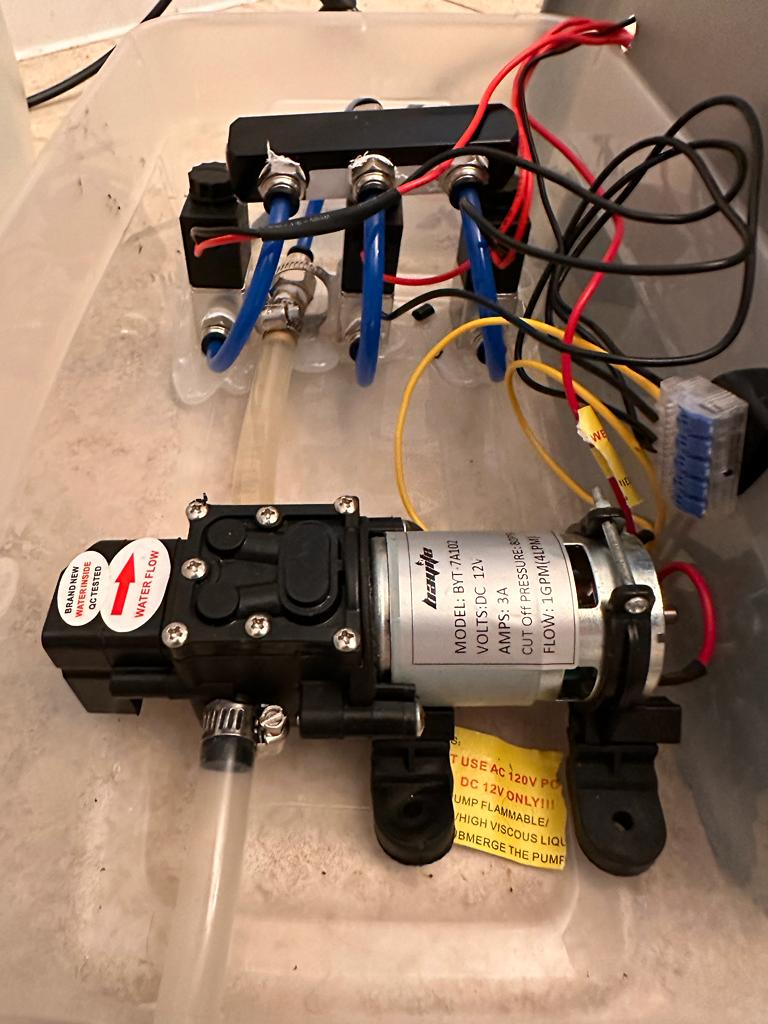
\includegraphics[width=0.5\textwidth]{./Figures/chapter4/pump_2.jpg}
	\caption[Conexión de bomba y válvulas]{Conexión de bomba y válvulas.}
	\label{fig:pump}
\end{figure}

\begin{figure}[!htpb]
     \centering
     \begin{subfigure}[b]{0.45\textwidth}
		\centering
		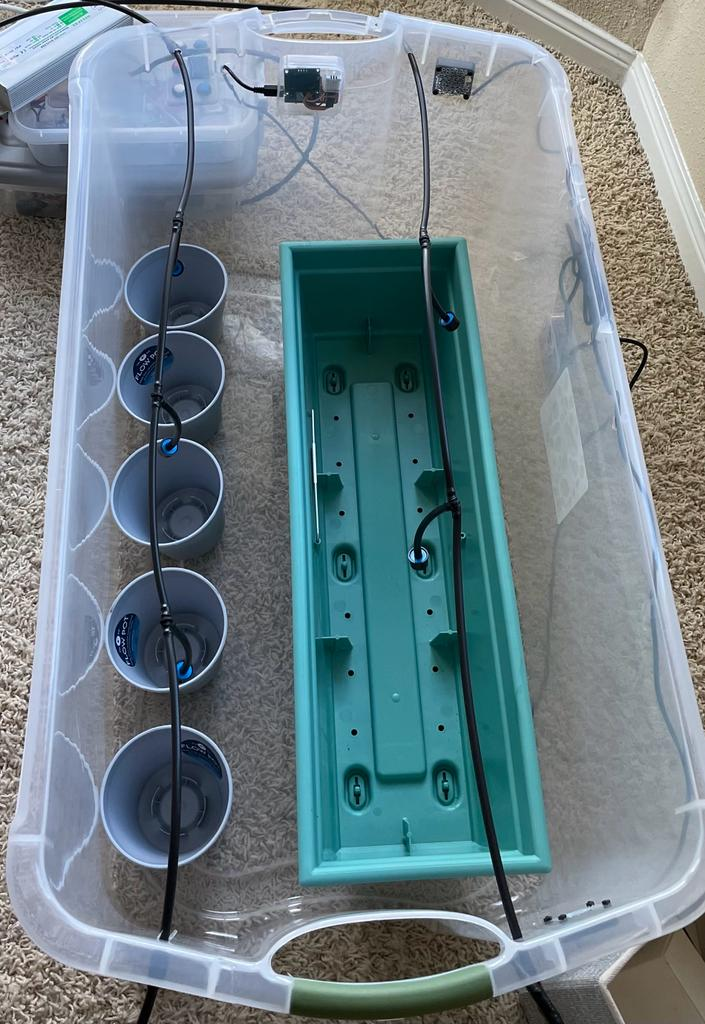
\includegraphics[width=0.70\textwidth]{./Figures/chapter4/Invernadero1.jpg}
		\caption{Armado de mangueras de riego.}
		\label{fig:gh1}
     \end{subfigure}
     \hfill
     \begin{subfigure}[b]{0.45\textwidth}
	    \centering
		 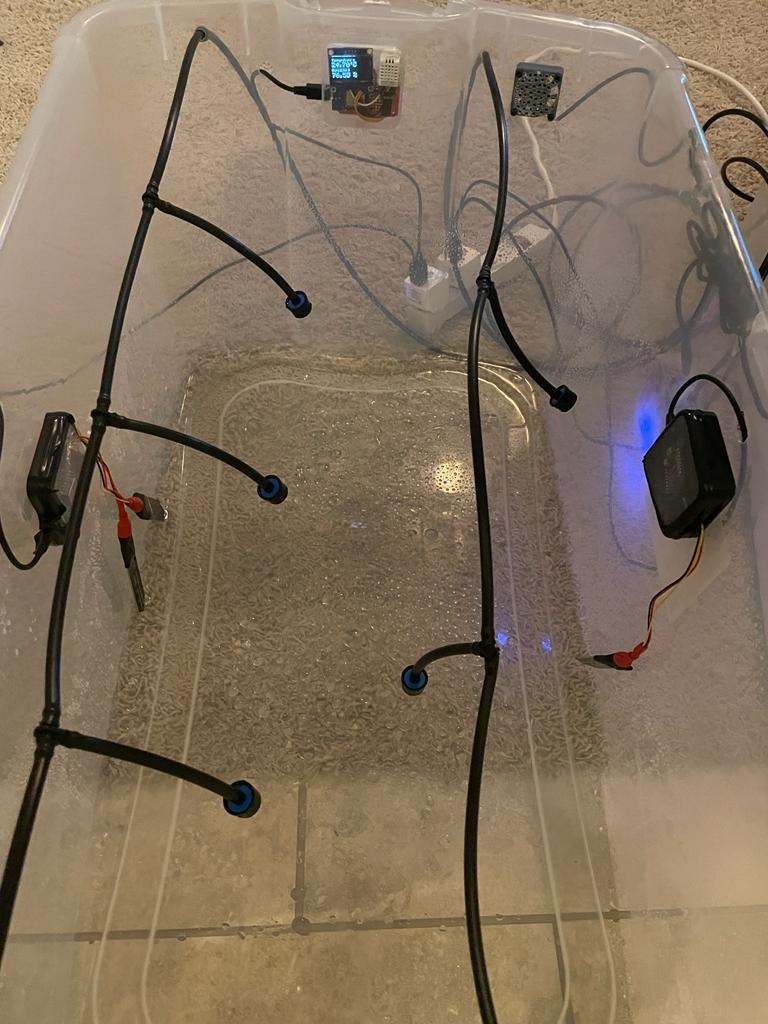
\includegraphics[width=0.75\textwidth]{./Figures/chapter4/Invernadero2.jpg}
		\caption{Pruebas de riego.}
		\label{fig:gh2}
     \end{subfigure}
     \hfill	
	 \begin{subfigure}[b]{0.45\textwidth}
		\centering
		\includegraphics[width=0.60\textwidth]{./Figures/chapter4/Invernadero3.jpg}
		\caption{Ensamble general.}
		\label{fig:gh3}
     \end{subfigure}
     \hfill
          \begin{subfigure}[b]{0.45\textwidth}
		\centering
		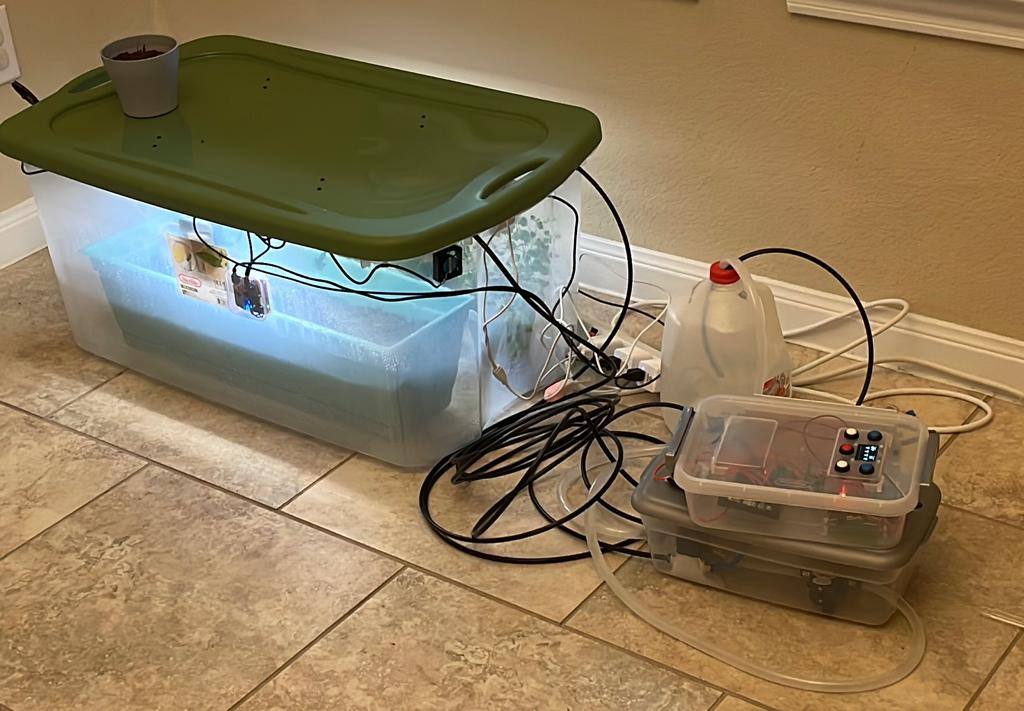
\includegraphics[width=0.90\textwidth]{./Figures/chapter4/Invernadero4.jpg}
		\caption{Modelo terminado.}
		\label{fig:gh4}
     \end{subfigure}
     \hfill
     \begin{subfigure}[b]{0.45\textwidth}
	    \centering
		 \includegraphics[width=0.80\textwidth]{./Figures/chapter4/Invernadero5.jpg}
		\caption{Modelo terminado.}
		\label{fig:gh5}
     \end{subfigure}
     \hfill	

        \caption[Modelo de pruebas del invernadero]{Modelo de pruebas del invernadero.}
        \label{fig:invernadero}
\end{figure}





\section{Pruebas unitarias}
\label{sec:Pruebas unitarias}
\section{Pruebas de sistema}
\label{sec:Pruebas de sistema}
\section{Comparativa con el estado de arte}
\label{sec:Comparativa con el estado de arte}